\documentclass{beamer}

\usetheme{CambridgeUS}

\usepackage[utf8x,utf8]{inputenc} % make weird characters work
\usepackage[serbian]{babel}

\usepackage{graphicx}
\graphicspath{{../images/}}
\usepackage{color}

\usepackage{verbatim}

\title{C++ Jezgro za Jupyter Notebook}
\subtitle{Interaktivno kuckanje u jeziku C++}

\author{G.~Vinterhalter \and M.~Ranković}

\institute[Beogradski univerzitet] 
{
  Matematički fakultet, Beogradski univerzitet\\
  (Metodologija stručnog i naučnog rada)
  }

\date{Prezentacija radova, 2016}

\subject{Metodologija Stručnog i Naučnog rada}
% This is only inserted into the PDF information catalog. Can be left
% out. 

% If you have a file called "university-logo-filename.xxx", where xxx
% is a graphic format that can be processed by latex or pdflatex,
% resp., then you can add a logo as follows:

% \pgfdeclareimage[height=0.5cm]{university-logo}{university-logo-filename}
% \logo{\pgfuseimage{university-logo}}


% Delete this, if you do not want the table of contents to pop up at
% the beginning of each subsection:

% \AtBeginSubsection[]
% {
%   \begin{frame}<beamer>{Outline}
%     \tableofcontents[currentsection,currentsubsection]
%   \end{frame}
% }

% Let's get started
\begin{document}

\begin{frame}
  \titlepage
\end{frame}

% \begin{frame}{Outline}
%   \tableofcontents
%   % You might wish to add the option [pausesections]
% \end{frame}

% Section and subsections will appear in the presentation overview
% and table of contents.
\section{Jupiter Notebook}

\subsection{Uvod}

\begin{frame}{Šta je to Jupyter Notebook ???}

  \quad Jupyter Notebook je web aplikacija za kreiranje i deljenje dokumenata
  koji pored uobičajenog tekstualnog sadržaja sadrže i interaktivni kod. 
  \pause


  \begin{itemize}
  \item {
      Dokument se sastoji iz vertikalnih ćelija: \pause
      \begin{itemize}
        \item ćelije teksta (markdown + latex math)
        \item ćelije koda  (kod koji Kernel izvršava)
        \item sirove ćelije
      \end{itemize}
      \pause
  }
  \item {
      Svaka ćelija se može izvršiti (osvežiti) zasebno,
      pri čemu ćelije koda imaju izlaz. 
      \pause
  }
  \item {
      Dokument se prikazuje renderuje kao html stranica. Zato izlaz može
      da predstavlja html kod. \pause
      \begin{itemize}
        \item Lepo formatiran kod
        \item slike, grafikoni (svg, png, jpg, ...)
        \item interaktivni sadržaj (java script)
      \end{itemize}

      \pause
  }
  \item{
      Ćelije podržavaju interaktivnu potržnju za korisničkim unosom.
    }
  \end{itemize}
\end{frame}

\subsection{Notebook format}

\begin{frame}{Format i konverzije}
  \begin{itemize}
  \item {
      Interno dokument se čuva kao ".json" fajl.
      (.ipynb format) \pause 
  }
  \item{
    \begin{figure}[h!]
    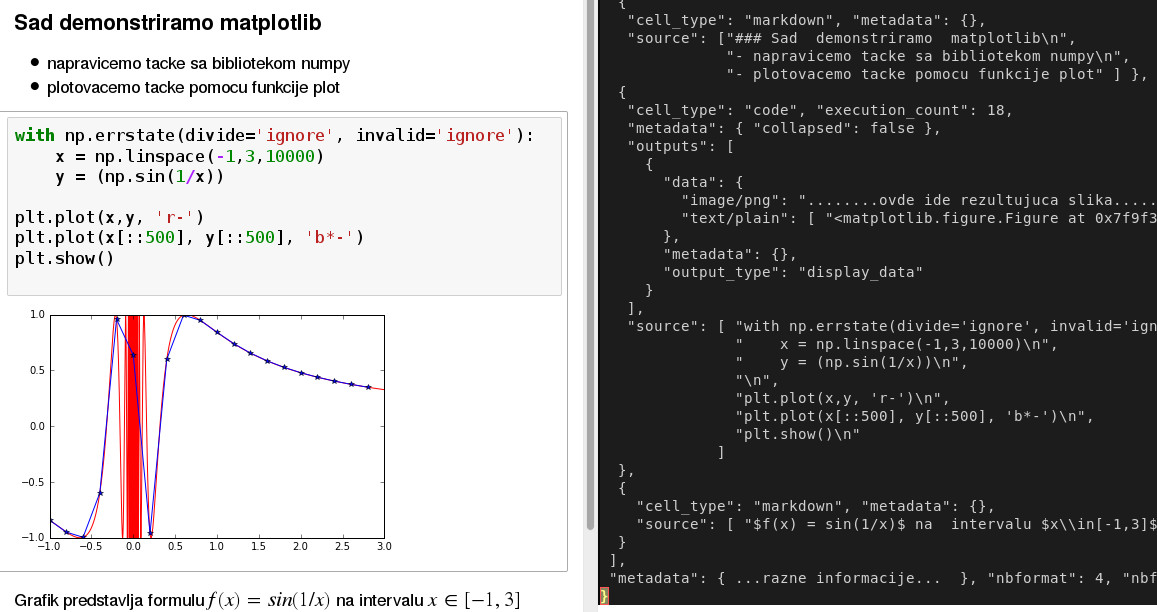
\includegraphics[scale=1]{nbPrimer_croped.jpg}
    \end{figure}
    \pause 
  }
  \item {
      Čuvaju se i izlazi ćelija \pause 
  }
  \item {   
      Dokument se može eksportovati : 
      {pdf (preko latexa)}, {html}, {html kao prezentacija},
       {markdown}, {izvrni kod}
      )
  }
  \end{itemize}
\end{frame}


\section {Arhitektura}

\subsection {Uvod u Arhitekturu}

\begin{frame}{Arhitektura}
\begin{itemize}
  \item{ arhitektura je klijent server. \pause 
          \begin{figure}[h!]
          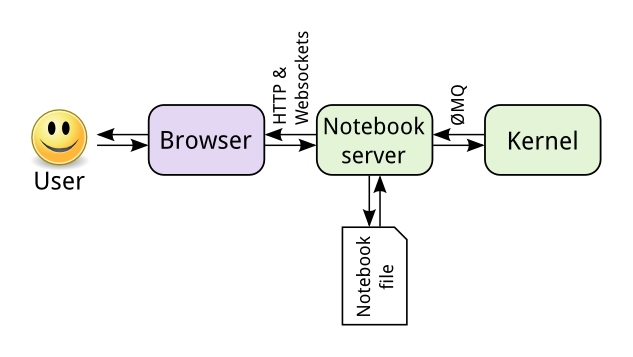
\includegraphics[scale=0.5]{nbKomponente.png}
          \end{figure}
          \pause
        }
\item{ Notebook server i Kernel (Jezgro) čine serverski deo aplikacije \pause }
  \item { Jezgro izvršava sadržaj ćelija koda. Jezgro obično podržava
          samo jedan jezik (Python, Haskell, Jullia, R, ...) \pause }
  \item {Mi želimo Jezgro koje će izvršavati C++ }
\end{itemize}

\end{frame}

\begin{frame}[fragile]{Dužnost Jezgra}
  \begin{itemize}
    \item {
        jezgro komunicira sa Notebook Server applikacijom i mora da ispoštuje
        određen format komunikacije (propisane poruke) \pause
      }
    \item{ Struktura poruke:
        \small
\begin{verbatim}
{
  'header' :{
    'msg' : uuid,
    'username' : str,
    'session' : uuid,
    'msg_type' : str,
    'version' : 5.0
  }

  'parent_header' : dict,
  'metadata' : dict,
  'content' : dict
}
\end{verbatim}
      }
  \end{itemize}
\end{frame}

\begin{frame}[fragile]{Bitne poruke}
  \begin{itemize}
    \item{ shell ROUTER/DEALER soket
        \begin{itemize}
          \item { execute\_request / reply }
          \item { introspect\_request / reply }
          \item { completion\_request / reply }
          \item { History\_request / reply }
          \item { KernelInfo\_request / reply }
          \item {...}
        \end{itemize}
      }

    \item{ PUB/SUB soket
        \begin{itemize}
          \item { stream (stdout, stderr, ...) }
          \item { display (html, svg, png, ..)}
          \item { clearOutput }
          \item { ... }
        \end{itemize}
      }

    \item{ stdin ROUTER/DEALER soket
        \begin{itemize}
          \item { input\_request }
        \end{itemize}
      }

    \item{ Dozvoljeno je dodavanje drugih vrsta poruka... }

  \end{itemize}
\end{frame}

\section {C++ Jezgro}

\begin{frame}[fragile]{Ideja za C++}
  \begin{itemize}

    \item{ Šta želimo?
        \begin{itemize}
          \item{Korisnik ima osećaj kao da radi sa skript jezikom}
          \item{Tačnije, promene u jednoj ćeliju utiču na ostale }
        \end{itemize}
        \pause
      }

    \item{ Koristimo dinamičko učitavanje. Ćeliju izvršavamo
        tako što: \pause
        \begin{itemize}
          \item{Kompjaliramo: \verb|g++ -shared -fpic| \pause}
          \item{U pythonu učitavamo .so preko CDLL f-je.
            (dlopen u pozadini) \\
            flagovi: \verb|RTLD_GLOBAL  RTLD_DEEPBIND|

          \pause}
          \item {pozivamo funkciju void \_\_run\_\_() koju smo prethodno
            ubacili u izvorni kod \pause}
        \end{itemize}
      }

    \item{  \verb|void __run__()|  se automatski generiše
        od strne C++ Jezgra i sadrži izraze koji nisu
        deklaracije/definicije. Koristmo specijalnu sintaksu koja
        je inače standardna za jupyter notebook jezgra  \pause
        \begin{itemize}
          \item{ \%r statment; line magic, statment je trenutno
            jednoliniski, U duhu c++ to bi trebalo prepraviti.}
          \item{ \%\%r statment;  cell magic, cela ćelija se
            smešta u \verb|void __run__()|}
        \end{itemize}
      }


  \end{itemize}


\end{frame}

\begin{frame}[fragile] {Primer 1}

  \fontsize{8pt}{0.2pt}


  \begin{columns}
    \column[t]{0.2cm}
\begin{verbatim}
1.
\end{verbatim}
    \column[t]{4.5cm}
\begin{verbatim}
int a = 10;
%r cout << a;
void f() {cout << a+1 << endl;}
\end{verbatim}
    \column[t]{4.5cm}
\begin{verbatim}
int a = 10;
void f() {cout << a+1 << endl;}
void__run__(){ cout << a; }
\end{verbatim}
    \column[t]{1.5cm}
\begin{verbatim}
result:
10
\end{verbatim}
  \end{columns}


    \begin{columns}
    \column[t]{0.1cm}
\begin{verbatim}
2.
\end{verbatim}
      \column[t]{4.5cm}
\begin{verbatim}
%rr
a = 25;
cout << a << endl;
f();
\end{verbatim}
      \column[t]{4.5cm}
\begin{verbatim}
extern int a;
void f();
void__run__(){ 
  a = 25;
  cout << a << endl; 
  f();
}
\end{verbatim}
    \column[t]{1.5cm}
\begin{verbatim}
result:
25
26
\end{verbatim}
    \end{columns}


    \begin{columns}
    \column[t]{0.1cm}
\begin{verbatim}
3.
\end{verbatim}
      \column[t]{4.5cm}
\begin{verbatim}
float a = 3.14;
%r cout << a << endl;
%r f();
\end{verbatim}
      \column[t]{4.5cm}
\begin{verbatim}
void f();
float a = 3.14;
void__run__(){ 
  cout << a << endl;
  f(); 
}
\end{verbatim}
    \pause
    \column[t]{1.5cm}
\begin{verbatim}
result:
3.14
26
\end{verbatim}
    \end{columns}
    \pause



    \begin{columns}
    \column[t]{0.1cm}
\begin{verbatim}
4.
\end{verbatim}
      \column[t]{4.5cm}
\begin{verbatim}
%rr
cout << a << endl;
f();
\end{verbatim}
      \column[t]{4.5cm}
\begin{verbatim}
extern float a;
void f();
void__run__(){ 
  cout << a << endl; 
  f();
}
\end{verbatim}
    \pause
    \column[t]{1.5cm}
\begin{verbatim}
result:
3.50325e-44
26
\end{verbatim}
    \end{columns}
% \end{block}

\end{frame}

\begin{frame}[fragile]{Rešenje}
  \begin{itemize}

    \item{ Funkcije menjamo pokazivačima na funkcije.
        \pause
        \begin{itemize}
          \item{funkciju \verb|void f() {...}| zamenjujemo pokazivačem
              tj. \verb|void f_1() {...} | \\ \verb|void (*f)() = f_1;|
            }
        \pause
      \item{Promena ponašanja funkcije (bez menjana potpisa) se svodi
        na promenu vrednosti  pokazivača.}
        \end{itemize}
        \pause
      }

    \item{ Redefinisanje tipova ili potpisa.
        \begin{itemize}
          \item{ Pravo ime je sakrivamo od korisnika. \pause
            }
          \item{ ako dođe do redefinicije menja se ime svim simbolima.
              Za sad jednostavno inkrementujem broj na kraju pravog
            imena. \pause
            }
          \item { Ime je promenjeno samo u toj ćeliji. U drugim ćelijma se idalje referiše staro ime jer nisu osvežene. Osvežavanje
              može da prozivede grešku jer se potpis više ne poklapa
              ili tip više ne podržava traženo ponašanje.
            }
        \end{itemize}
      }


  \end{itemize}


\end{frame}

\section{Clang}

\subsection{libclang}

\begin{frame}{libclang}

\begin{itemize}
  \item { libclang je C biblioteka koju koristimo za parsiranje C++
      koda.
  }
  \item { Biblioteka je napravljena da korisnik može da obilazi
    apstraktno stablo sintakse (eng. AST) krećući se kroz čvorove
    tako što registruje handler funkcije koje sam definiše.
  }
  \item { Osnovni element stabla je CXCursor i sadrži informacije:
      \begin{itemize}
        \item { tipu:
            \begin{itemize}
              \item {Razne vrste deklaracije}
              \item {Razne vrste  izraza}
              \item {Direktive}
              \item {i još mnogo toga ...}
            \end{itemize}
          }
        \item{ datoteka u kojoj se nalazi } (izbegavanje include fajlova)
      \item{ Lokacija u izvornom kodu } (pamtimo za modifikaciju koda)
      \item{ tip podataka (potipis, povratna vrednost) } (pamtimo)
      \item{ ime simbola } (pamtimo)
      \item{ kvalifikacioni atributi } (pamtimo)
      \item{ referenca na definiciju } (prepoznavanje lokalnih promenljivih)
      \end{itemize}

  }
\end{itemize}

\end{frame}


\begin{frame}[fragile]{libclang}


  Auto ?
\begin{itemize}
    \item{\verb|auto| je predstavljen Kursorom 'unresolved'}
    \item{Međutim već naredni Cursor sadrži potreban tip}
    \item{U slučaju \verb|const auto &|, prvi kursor je \verb|&|}
\end{itemize}

  \scriptsize
\begin{verbatim}
int * * a = nullptr;                                                            
auto b = 3.14;                                                                  
auto f(int  c) {return nullptr};
  ----------------------------------------
TranslationUnitDecl <<invalid sloc>> <invalid sloc>
|-VarDecl <t1.cpp:2:1, col:13> col:9 a 'int **' cinit
| `-ImplicitCastExpr <col:13> 'int **' <NullToPointer>
|   `-CXXNullPtrLiteralExpr <col:13> 'nullptr_t'
|-VarDecl <line:4:1, col:10> col:6 b 'double':'double' cinit
| `-FloatingLiteral 0x25b0c58 <col:10> 'double' 3.140000e+00
|-FunctionDecl <line:5:1, col:31> col:6 f 'void* (int)'
| |-ParmVarDecl <col:8, col:13> col:13 c 'int'
| `-CompoundStmt <col:16, col:31>
|   `-ReturnStmt <col:17, col:24>
|     `-CXXNullPtrLiteralExpr <col:24> 'nullptr_t'
`-EmptyDecl <col:32> col:32
\end{verbatim}

\end{frame}






\section{Kraj}

\begin{frame}{Kraj}
  \begin {itemize}
\item{ Nedostaci:
    \begin{itemize}
    \item {Trenutno ne podržavamo klase/strukture, unije i šablone.}
    \item {Segmentation Fault ubija jezgro.}
    \item {Interaktivni  unos korisnika fali.}
    \item {Nisu sve poruke implementirane.}
  \end{itemize}
    }


  \item{ Literatura:
      \begin{itemize}
\item {
Ipython Developer documentation \\
    \scriptsize
\url{https://ipython.org/ipython-doc/3/development/}
}

\item {
Ipython magic documentation \\
    \scriptsize
\url{ https://ipython.org/ipython-doc/3/interactive/magics.html }
}

\item {
dlopen man page 
    \scriptsize
\url{ http://linux.die.net/man/3/dlopen}
}


\item {
Jupyter project 
    \scriptsize
\url{http://jupyter.org/}
}

\item {
Clang documentation 
    \scriptsize
\url{http://clang.llvm.org/}
}

\item {
Linkers and Loaders,  John R. Levine \\
    \scriptsize
% \url{http://www.amazon.com/Linkers-Kaufmann-Software-Engineering-Programming/dp/1558604960}
}
      \end{itemize}
}
  \end {itemize}
  
\end{frame}


\end{document}


